% Copyright 2026 Sreeram Anil
% SPDX-License-Identifier: CC-BY-4.0
% =============================================================================
%  Iterated posterior linearisation filter — classical Kalman family
% =============================================================================
\chapter{Iterated Posterior Linearisation Filter (IPLF)}
\label{ch:iplf}

\section*{At a glance}
\begin{tabular}{@{}l>{\raggedright\arraybackslash}p{0.76\textwidth}@{}}
Family & classical Kalman (sigma-point, iterated) \\
Header & \texttt{include/estkit/filters/iplf.hpp} \\
Registered name & \texttt{IPLF} \\
State dimension & $n_x = 4$ (cell model) --- generic in $n_x, n_u, n_y$ \\
Sigma points & $2n_x+1 = 9$ per iteration, $\le 5$ iterations \\
Cost per step & $\mathcal{O}(J n_x^3)$ plus $(J{+}1)(2n_x{+}1)$ model calls; $1.92$--$2.08\,\SI{}{\micro\second}$/step \\
Primary references & \cite{garciafernandez2015iplf,garciafernandez2017ipls,julier2000newmethod,bellcathey1993} \\
\end{tabular}

\section{Motivation and aerospace/BMS relevance}
Two ideas have appeared separately in this family. The sigma-point filters replace the
Jacobian by a \emph{statistical linear regression} (SLR) of $h$ taken with respect to the
\emph{prior}; the iterated EKF keeps the analytic Jacobian but moves the expansion point to
the \emph{posterior}. García-Fernández, Svensson, Morelande and
Särkkä~\cite{garciafernandez2015iplf} observed that the two are orthogonal improvements and
combined them: perform the SLR with respect to the current posterior approximation and
iterate.

The argument for doing so is precise. The best linear approximation of $h$ in a mean-square
sense depends on the density with respect to which the error is measured. A filter should
linearise where the state actually \emph{is} (the posterior), not where it was believed to be
before the measurement (the prior). When the measurement is informative --- and a battery
terminal-voltage measurement with $\sigma_v = 2$\,mV against an OCV slope of $0.8$\,V is very
informative --- the posterior is far narrower than the prior, and a regression over the
prior wastes its accuracy on regions of the state space the measurement has just excluded.

For BMS the practical case is again initialisation and fault recovery, and for GNC it is the
classic one of a very accurate sensor with a nonlinear model (range, bearing, star tracker).

\section{Problem statement and assumptions}
Model \eqref{eq:ekf-proc}--\eqref{eq:ekf-meas}, additive noise. Given a Gaussian prior
$\N{\xminus_k}{\Pminus_k}$ and a measurement $\vy_k$, the goal is the Gaussian
$\N{\vx_J}{\mP_J}$ that best approximates the true posterior in Kullback--Leibler divergence.
The filter assumes a Gaussian posterior; it makes no differentiability assumption on $h$.

\begin{definition}[Statistical linear regression]\label{def:slr}
Given a density $p(\vx)$ with mean $\bar\vx$ and covariance $\bar\mP$, the SLR of $h$ with
respect to $p$ is the triple $(\mA,\bm{b},\bm{\Omega})$ minimising
$\E{\norm{h(\vx)-(\mA\vx+\bm{b})}^2}$ under $p$, together with the covariance
$\bm{\Omega}$ of the residual $h(\vx)-(\mA\vx+\bm b)$.
\end{definition}

\section{Derivation}
\paragraph{Closed form of the SLR.} Writing
$\bar{\vy} = \E{h(\vx)}$, $\bm{\Psi} = \E{(\vx-\bar\vx)(h(\vx)-\bar\vy)^\T}$ and
$\bm{\Phi} = \E{(h(\vx)-\bar\vy)(h(\vx)-\bar\vy)^\T}$, the first-order conditions of the
least-squares problem in Definition~\ref{def:slr} give
\begin{equation}
\mA = \bm{\Psi}^\T\bar{\mP}\inv, \qquad
\bm{b} = \bar{\vy} - \mA\bar{\vx}, \qquad
\bm{\Omega} = \bm{\Phi} - \mA\bar{\mP}\mA^\T,
\label{eq:iplf-slr}
\end{equation}
with $\bm{\Omega}\succeq 0$ by construction (it is the covariance of the part of $h$ that no
affine function of $\vx$ can explain). The three moments $\bar\vy,\bm\Psi,\bm\Phi$ are
evaluated with the sigma-point rule of Chapter~\ref{ch:ukf}; any of the rules in this family
would do.

\paragraph{The iteration.} Initialise $\vx_0 = \xminus_k$, $\mP_0 = \Pminus_k$. For
$j=0,1,\dots$: compute the SLR $(\mA_j,\bm b_j,\bm\Omega_j)$ of $h$ with respect to
$\N{\vx_j}{\mP_j}$ using \eqref{eq:iplf-slr}, then update the \emph{prior} with the resulting
affine measurement model $\vy = \mA_j\vx + \bm b_j + \bm{e}$,
$\bm{e}\sim\N{\bm0}{\bm\Omega_j + \mR}$:
\begin{align}
\mS_j &= \mA_j\Pminus_k\mA_j^\T + \bm\Omega_j + \mR, &
\mK_j &= \Pminus_k\mA_j^\T\mS_j\inv, \label{eq:iplf-gain}\\
\vx_{j+1} &= \xminus_k + \mK_j\left(\vy_k - \mA_j\xminus_k - \bm b_j\right), &
\mP_{j+1} &= \Pminus_k - \mK_j\mS_j\mK_j^\T. \label{eq:iplf-update}
\end{align}
It is essential that \eqref{eq:iplf-update} updates the \emph{original} prior
$(\xminus_k,\Pminus_k)$, not $(\vx_j,\mP_j)$: the iteration changes only where the
measurement model is linearised, never how much information has been used.

\begin{proposition}[One iteration is the sigma-point filter]\label{prop:iplf-first}
With $\vx_0 = \xminus_k$, $\mP_0=\Pminus_k$, \eqref{eq:iplf-gain}--\eqref{eq:iplf-update}
reduce exactly to the UKF measurement update \eqref{eq:ukf-pyy}--\eqref{eq:ukf-mu}.
\end{proposition}
\begin{proof}
With $\bar\mP = \Pminus_k$, $\bm\Omega_0 = \bm\Phi - \mA_0\Pminus_k\mA_0^\T$, hence
$\mS_0 = \bm\Phi + \mR = \mP_{yy}$. Also
$\mK_0 = \Pminus_k\mA_0^\T\mS_0\inv = \Pminus_k(\Pminus_k)\inv\bm\Psi\,\mP_{yy}\inv =
\mP_{xy}\mP_{yy}\inv$, and
$\vy_k - \mA_0\xminus_k-\bm b_0 = \vy_k - \bar\vy = \vy_k-\yhat_k$. Substituting gives
\eqref{eq:ukf-mu}.
\end{proof}
Proposition~\ref{prop:iplf-first} was verified numerically: with \code{max\_iter = 1} the IPLF
and the library UKF agree to $\max\abs{\Delta\vx} = 4.0\times10^{-11}$ over a full mission.

\paragraph{Interpretation and convergence.} García-Fernández et
al.~\cite{garciafernandez2015iplf} show that \eqref{eq:iplf-gain}--\eqref{eq:iplf-update} is a
fixed-point iteration whose fixed points are the stationary points of the KL divergence
between the true posterior and the Gaussian family, and that the IEKF
(Chapter~\ref{ch:iekf}) is recovered if the SLR in \eqref{eq:iplf-slr} is replaced by a Taylor
linearisation at $\vx_j$ --- the IPLF is the IEKF with derivatives replaced by regressions
and, crucially, with $\bm\Omega_j$ accounting for the part of $h$ that no linearisation can
capture. Convergence is not guaranteed in general; as with Gauss--Newton the practical
remedy is a small iteration budget, used here.

\section{Algorithm}
\begin{algorithm}[H]
\caption{IPLF --- one sampling period}
\begin{algorithmic}[1]
\Require $\xplus_{k-1},\Pplus_{k-1},\vu_{k-1},\vy_k,\vu_k$, $J_{\max}$, tolerance $\epsilon$
\State \textbf{Time update:} sigma-point prediction \eqref{eq:ukf-tu-mean}--\eqref{eq:ukf-tu-cov} $\Rightarrow (\xminus_k,\Pminus_k)$
\State $\vx_0\gets\xminus_k$, $\mP_0\gets\Pminus_k$
\For{$j=0,\dots,J_{\max}-1$}
  \State generate sigma points from $(\vx_j,\mP_j)$; $\mathcal{Z}_i\gets h(\mathcal{X}_i,\vu_k)$
  \State $\bar\vy\gets\sum_i W^m_i\mathcal{Z}_i$;\;
         $\bm\Psi\gets\sum_i W^c_i(\mathcal{X}_i-\vx_j)(\mathcal{Z}_i-\bar\vy)^\T$;\;
         $\bm\Phi\gets\sum_i W^c_i(\mathcal{Z}_i-\bar\vy)(\cdot)^\T$
  \State $\mA\gets\bm\Psi^\T\mP_j\inv$ (Cholesky solve);\; $\bm b\gets\bar\vy-\mA\vx_j$;\;
         $\bm\Omega\gets\bm\Phi-\mA\mP_j\mA^\T$, clipped to $\succeq0$
  \State $\mS\gets\mA\Pminus_k\mA^\T+\bm\Omega+\mR$;\; $\mK\gets\Pminus_k\mA^\T\mS\inv$
  \State $\vx_{j+1}\gets\xminus_k+\mK(\vy_k-\mA\xminus_k-\bm b)$;\;
         $\mP_{j+1}\gets\Pminus_k-\mK\mS\mK^\T$
  \State \textbf{if} $\norm{\vx_{j+1}-\vx_j}\le\epsilon(1+\norm{\vx_{j+1}})$ \textbf{then break}
\EndFor
\State $\xplus_k\gets\vx_J$, $\Pplus_k\gets\mP_J$;
       \textbf{if} constraints enabled \textbf{then} $\xplus_k\gets\Pi(\xplus_k)$
\Ensure $\xplus_k,\Pplus_k$
\end{algorithmic}
\end{algorithm}

\section{Application to the battery model}
The regression matrix $\mA$ has a direct physical reading here: its first entry is the
\emph{effective OCV slope} averaged over the current posterior. During the first iteration
that average is taken over the prior ($\sigma_\soc$ up to $0.1$ at start-up) and is the chord
of the OCV curve; by the second iteration the posterior is already $30\times$ narrower and
the regression returns essentially the local tangent --- so the IPLF automatically interpolates
between the CKF's chord behaviour and the EKF's tangent behaviour as the measurement takes
effect. This is the cleanest available answer to the trade-off identified in
Chapters~\ref{ch:ckf} and~\ref{ch:ekf}.

The residual covariance $\bm\Omega$ is the second useful quantity: it is the variance of the
OCV nonlinearity that the affine fit cannot explain, and it is added to $\mR$, so the filter
automatically de-weights the voltage measurement while the SOC uncertainty is large. That is
the same inflation that the UKF obtains accidentally through a large negative $W_0^c$
(Remark~\ref{rm:ukf-w0}) and the second-order EKF obtains explicitly
(Chapter~\ref{ch:soekf}), but here it is derived rather than incidental.

Options: $\alpha=0.1,\beta=2,\kappa=0$ (matching the UKF so that
Proposition~\ref{prop:iplf-first} can be checked), \code{max\_iter = 5},
\code{tol}$=10^{-6}$, \code{apply\_constraints = true}.

\section{Implementation notes}
$\mA = \bm\Psi^\T\mP_j\inv$ is computed as $(\,\code{solve\_spd}(\mP_j,\bm\Psi)\,)^\T$, never
by forming an explicit inverse; if the Cholesky solve fails the iteration breaks and the last
valid iterate is kept. $\bm\Omega$ is clipped to a non-negative diagonal and symmetrised,
which guards against the small negative values that sigma-point moment sums with negative
$W_0^c$ can produce. Sigma points are regenerated from $(\vx_j,\mP_j)$ at every iteration ---
that is the whole point of the algorithm --- so the cost is $(J+1)\times 9$ model
evaluations; the measured $1.92$--$2.08\,\SI{}{\micro\second}$ per step implies an average of
about two iterations. \code{sizeof(Iplf<EcmModel>)} is 4784\,bytes.

\section{Benchmark results}
% Copyright 2026 Sreeram Anil
% SPDX-License-Identifier: CC-BY-4.0
\begin{table}[H]\centering\footnotesize\setlength{\tabcolsep}{4pt}
\caption{IPLF: cell-level benchmark on the eVTOL mission (mean over seeds; RMSE and max error in \% SOC; $t_\mathrm{conv}$: first time the error stays below 2\,\% for 60\,s, -- = never; EKF reference: steady-state RMSE of the plain EKF on the same data).}\label{tab:cell_IPLF}
\begin{tabular}{llrrrrrcrr}\toprule
plant & scenario & RMSE & RMSE$_\mathrm{ss}$ & max & $t_\mathrm{conv}$ [s] & RMSE$_v$ [mV] & div. & EKF ref. & ns/step \\ \midrule
ECM & nominal & 0.36 & 0.08 & 3.57 & 0 & 1.09 & no & 0.05 & 2032 \\
ECM & init\_error & 0.32 & 0.07 & 1.17 & 0 & 2.05 & no & 0.05 & 2033 \\
ECM & current\_bias & 0.70 & 0.57 & 3.35 & 0 & 1.12 & no & 0.61 & 2042 \\
ECM & noise\_step & 0.39 & 0.19 & 3.57 & 0 & 2.98 & no & 0.12 & 2077 \\
ECM & outliers & 0.94 & 0.26 & 5.77 & 174 & 2.23 & no & 0.21 & 2025 \\
ECM & cold & 0.54 & 0.50 & 3.53 & 0 & 2.03 & no & 0.16 & 2041 \\
ECM & hot & 0.44 & 0.02 & 3.59 & 0 & 0.92 & no & 0.03 & 2040 \\
ECM & aged\_cell & 1.83 & 2.16 & 4.66 & 0 & 3.99 & no & 1.52 & 2050 \\
ECM & param\_mismatch & 0.65 & 0.53 & 4.65 & 0 & 2.95 & no & 1.36 & 2067 \\
ECM & sensor\_dropout & 1.27 & 0.79 & 4.22 & 0 & 1.89 & no & 0.46 & 2047 \\
ECM & preisach & 0.49 & 0.20 & 3.66 & 1 & 1.16 & no & 0.20 & 2058 \\
ECM & combined & 1.49 & 1.72 & 4.90 & 0 & 4.67 & no & 12.44 & 2078 \\
\midrule
SPM & nominal & 3.65 & 3.74 & 4.39 & 0 & 1.30 & no & 3.73 & 1946 \\
SPM & init\_error & 3.94 & 4.01 & 4.68 & 0 & 2.11 & no & 3.81 & 1920 \\
SPM & current\_bias & 5.56 & 6.31 & 7.16 & 0 & 1.37 & no & 5.69 & 1940 \\
SPM & noise\_step & 4.70 & 5.55 & 8.61 & 0 & 3.26 & no & 3.30 & 2003 \\
SPM & outliers & 1.38 & 1.02 & 4.77 & 70 & 2.44 & no & 1.99 & 1922 \\
SPM & cold & 7.19 & 7.54 & 9.99 & -- & 4.59 & no & 7.35 & 1939 \\
SPM & hot & 2.25 & 2.33 & 3.55 & 0 & 1.04 & no & 2.16 & 1933 \\
SPM & param\_mismatch & 3.38 & 3.68 & 4.27 & 0 & 2.12 & no & 3.13 & 1922 \\
SPM & sensor\_dropout & 6.07 & 6.30 & 6.80 & 0 & 2.09 & no & 5.31 & 1924 \\
\bottomrule\end{tabular}\end{table}

\begin{figure}[H]\centering
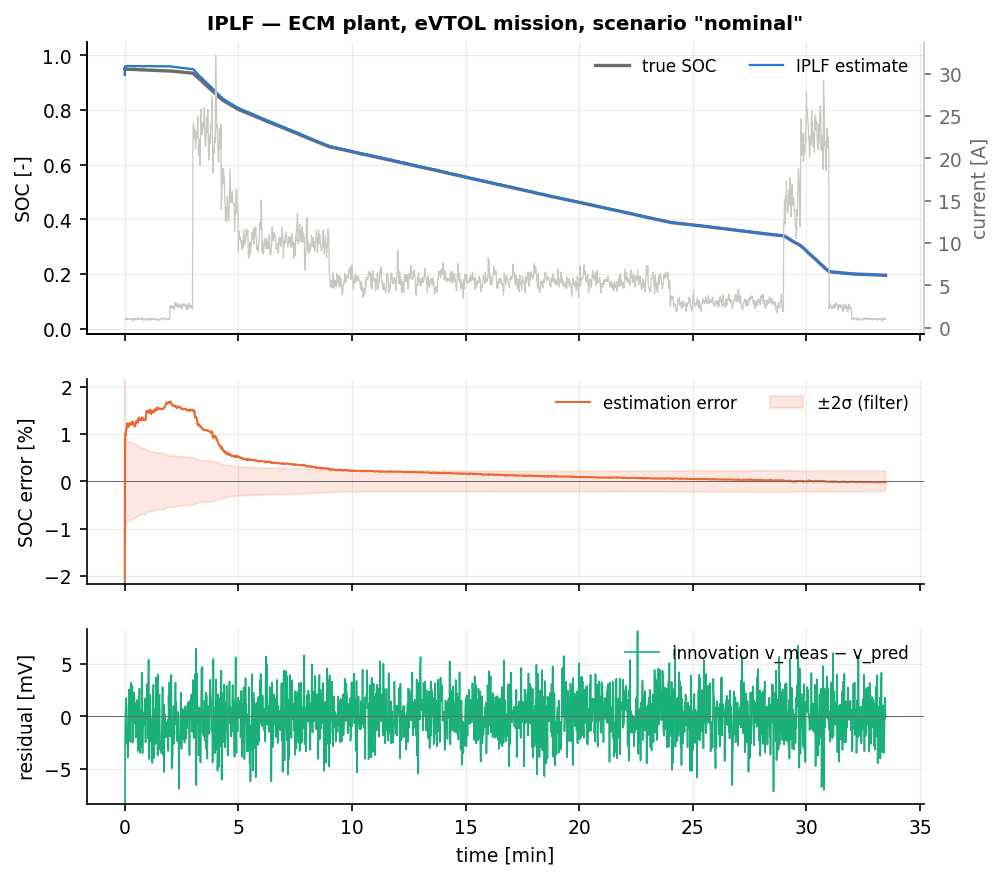
\includegraphics[width=\textwidth]{figures/cell_IPLF_nominal.png}
\caption{IPLF on the nominal eVTOL mission: true and estimated SOC (top), estimation error with the $\pm 2\sigma$ band when available (middle), voltage residual (bottom).}
\end{figure}
\begin{figure}[H]\centering
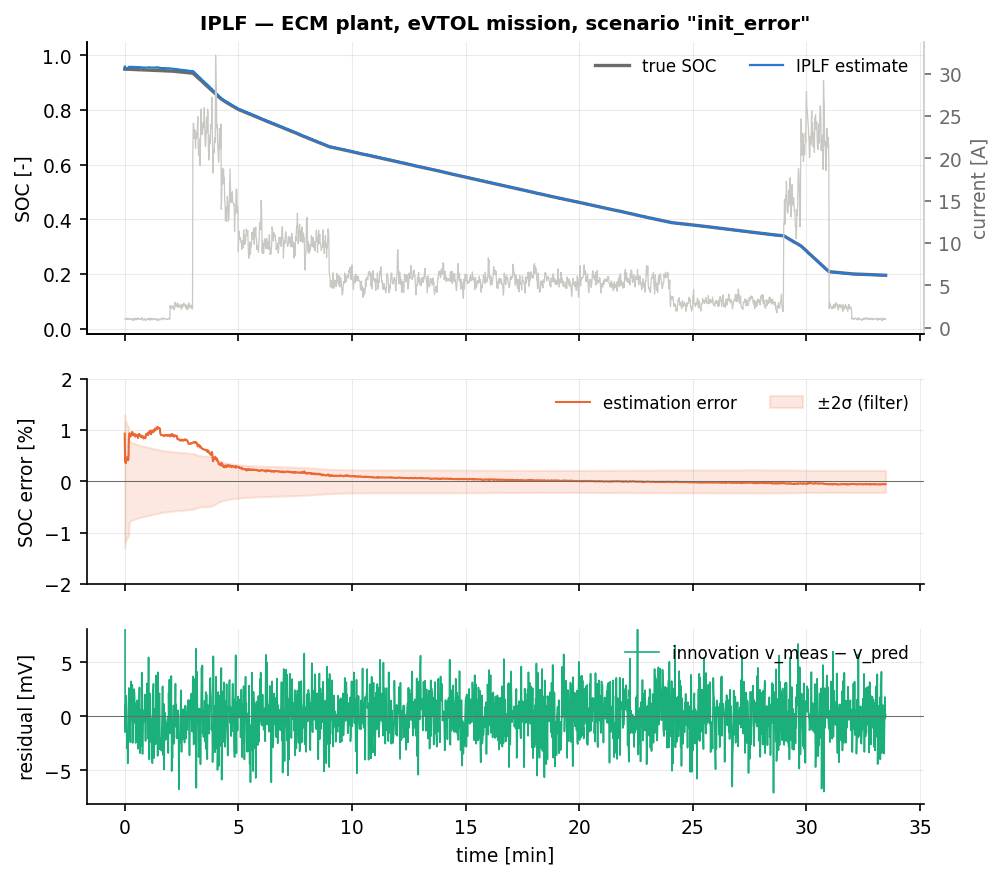
\includegraphics[width=\textwidth]{figures/cell_IPLF_init_error.png}
\caption{IPLF with a 35\,\% initial SOC error.}
\end{figure}
\begin{figure}[H]\centering
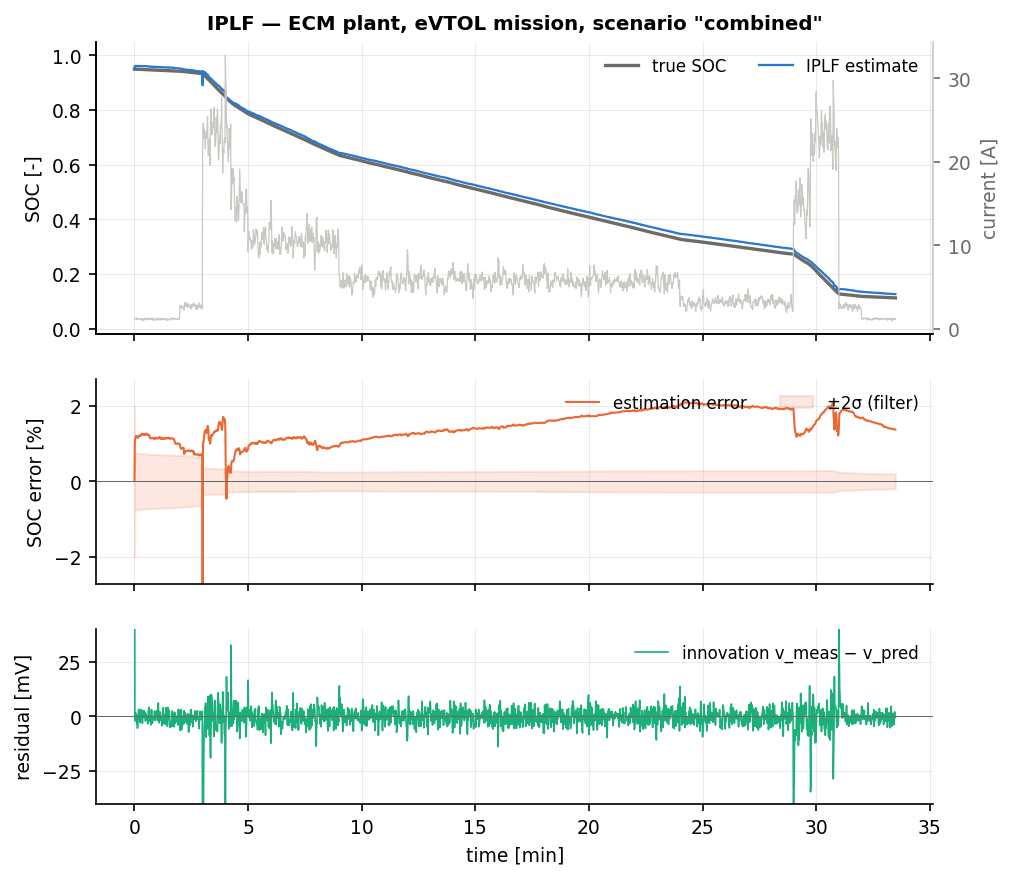
\includegraphics[width=\textwidth]{figures/cell_IPLF_combined.png}
\caption{IPLF on the \texttt{combined} scenario: the regression residual covariance $\bm\Omega$ de-weights the voltage while $\sigma_\soc$ is large, and the filter converges in the first sample.}
\end{figure}

All numbers are three-seed means in per cent SOC.

The IPLF has the best steady-state accuracy of any filter in the family on the two scenarios
that punish a bad linearisation hardest. \texttt{param\_mismatch} gives $0.65/0.53\,\%$ ---
the best of all fifteen, against the EKF's $1.28/1.36\,\%$, the UKF's $1.29/1.37\,\%$ and the
SO-EKF's $0.77/0.89\,\%$ --- and \texttt{hot} $0.02\,\%$, also the best. On \texttt{combined}
it converges in the first sample and reaches $1.49/1.72\,\%$, in the same class as the UKF
($1.19\,\%$) and the SO-EKF ($1.28\,\%$) and far better than the EKF ($12.44\,\%$); on
\texttt{init\_error} it converges immediately with $0.32/0.07\,\%$ where the CKF, CKF5, CDKF
and GHKF all need over $220$\,s. \texttt{preisach} is the fastest convergence of the fifteen
($1$\,s, against $16$\,s for the EKF and $214$--$229$\,s for the sigma-point filters) at
$0.49/0.20\,\%$ --- the regression absorbs the hysteresis offset immediately instead of
waiting for the covariance to reopen.

The whole-run RMSE on \texttt{nominal} ($0.36\,\%$ against the EKF's $0.15\,\%$, steady state
$0.08\,\%$ against $0.05\,\%$) and the convergence metric are the cost of that behaviour. In
the first seconds $\bm\Omega$ is large --- the OCV nonlinearity over $\sigma_\soc = 0.1$ is
genuinely un-modellable by an affine fit --- so the filter deliberately distrusts the first
voltage samples. That is correct behaviour, not a defect; the same caution is what makes
\texttt{combined} and \texttt{param\_mismatch} work.

Two clear regressions. \texttt{aged\_cell} is $1.83/2.16\,\%$ against the EKF's
$1.18/1.52\,\%$ and the CKF5's $2.50/1.54\,\%$ --- the worst steady-state figure of the family
apart from the LKF. With a $15\,\%$ capacity loss the model is simply wrong, the innovations
are persistently biased, and iterating the linearisation onto a posterior that is itself biased
reinforces the error. \texttt{cold} shows the same pattern on a smaller scale ($0.50\,\%$
against the UKF's $0.07\,\%$ and the EKF's $0.16\,\%$), as does \texttt{outliers}
($0.94/0.26\,\%$, with $t_{\text{conv}} = 174$\,s) --- fitting a corrupted measurement
\emph{better} is not an improvement, the same structural objection that applies to the IEKF.

Iteration-count sensitivity measured during development: $J = 1$ reproduces the UKF exactly,
$J = 2$ gives the best \texttt{combined} figure, and $J = 3,5,10$ are non-monotone. As with the
IEKF, more iterations is not monotonically better once model error dominates.

\paragraph{SPM plant: structured model error.}
\begin{figure}[H]\centering
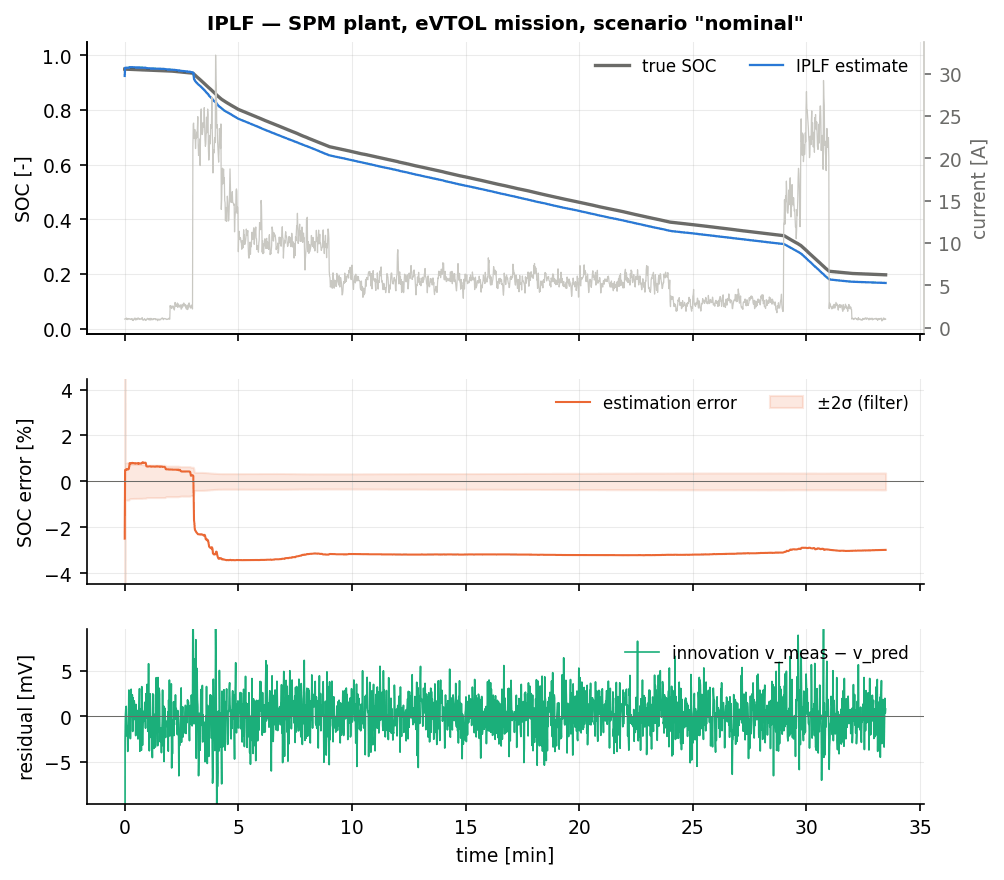
\includegraphics[width=\textwidth]{figures/cellspm_IPLF_nominal.png}
\caption{IPLF on the nominal mission with the electrochemical (SPM) plant.}
\end{figure}
The SPM block of the table is a different kind of test. The plant is the electrochemical
single-particle model; the estimator still runs a 2-RC equivalent circuit, fitted to that plant,
which leaves a \emph{structured} residual of about $4$\,mV (Butler--Volmer kinetics and
solid-phase diffusion that no 2-RC circuit can reproduce) and a slow second branch,
$\tau_2 = 556$\,s. Over a $33$-minute mission a $556$\,s pole barely relaxes, so $v_2(t)$ is
close to an affine ramp --- and so is $\ocv(\soc(t))$ while the cell discharges at a roughly
constant rate. The two channels through which the measurement sees the state,
$(\partial\ocv/\partial\soc)\,\delta\soc$ and $-\delta v_2$, are therefore nearly collinear in
the information accumulated over the flight: the pair $(\soc, v_2)$ is close to unobservable,
and no filter can decide whether a persistent few-millivolt residual belongs to the slow RC
branch or to the state of charge. Because that direction is weakly observable, a $4$\,mV
structured error maps onto \emph{several per cent} of SOC instead of the
$4\,\text{mV}/0.8\,\text{V}\approx0.5\,\%$ a well-conditioned channel would give. This
$(\soc,v_2)$ ambiguity, not the size of the residual, is the mechanism behind the
$3.7$--$4.6\,\%$ band in which the whole classical family sits.

The IPLF lands at $3.74\,\%$ on SPM \texttt{nominal}, essentially on top of the EKF's
$3.73\,\%$ and well ahead of the other sigma-point filters (UKF $3.96\,\%$, cubature family
$4.61$--$4.62\,\%$). That is the posterior linearisation doing what it is designed to do: after
the first iteration the regression is taken over a posterior that is $30\times$ narrower than
the prior, so the effective OCV slope is the local tangent rather than the chord, and the
filter does not over-weight the ill-conditioned channel the way a prior-based regression does.
It is the best SPM \texttt{outliers} result of the family by a wide margin ($1.02\,\%$ against
the EKF's $1.99\,\%$ and the cubature filters' $2.21$--$2.27\,\%$), because $\bm\Omega$ absorbs
exactly the part of the residual that no affine model explains.

What it does not do is escape the band. On \texttt{noise\_step} it is the worst of the fifteen
($5.55\,\%$ against the EKF's $3.30\,\%$): when the voltage noise steps up by an order of
magnitude the posterior stops being narrow, the regression widens again, and the filter
re-commits to the ambiguous direction. \texttt{sensor\_dropout} ($6.30\,\%$ against $5.31\,\%$)
and \texttt{current\_bias} ($6.31\,\%$ against $5.69\,\%$) show the same. Linearising in the
right place is worth about $6\,\%$ here; resolving the $(\soc,v_2)$ ambiguity would need an
extra state or a second sensor, not a better linearisation.

\section{Summary}
The IPLF is the most principled filter in this family: it linearises statistically, where the
state is, and it charges the linearisation residual $\bm\Omega$ to the measurement noise so
that the filter's confidence matches the quality of its own approximation. On this benchmark it
delivers the best steady-state accuracy on \texttt{param\_mismatch} and \texttt{hot}, the
fastest convergence on \texttt{preisach}, immediate convergence from a large initial error, and
it survives \texttt{combined}, at about $1.4\times$ the cost of a UKF. Use it when the
measurement is informative and strongly nonlinear. Do not expect it to help when the model
itself is biased --- on \texttt{aged\_cell} it is the worst of the sigma-point filters, and on
the SPM plant it merely matches the EKF --- because a better fit to a wrong model is still
wrong.
